\chapter{Experiments\&Results}

\section{Datasets}

We evalute our models on three different datasets.
The dataset size is primarily limited by the computational resources, such as memory and computation time. 

\subsection{1x4 Dataset}

The simplest dataset we use a 1 dimensional binary dataset of size 4, where either the first or the last element is set to 1. 

\begin{figure}
	\centering
    	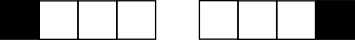
\includegraphics[width=0.7\textwidth]{imgs/1x4_ds.png} 
    \caption{A figure.}
	\label{fig:test}
\end{figure}

\subsection{Strip Dataset}

We generate a 10x10 pixel noisy stripe dataset, with three different oriented stripes, horizontal, diagonal, vertical. 

This could represent a similar object to a pen recorded with a event-based camera, and result in an grasp id.

In the easiest version of this dataset, the stripes always occur on the same places, with some random noise.

An more complex version of the datasets contains the stripes randomly distributed across the whole image.

The dataset can be either binary or continuous.

\subsection{MNIST}

We also evaluate the models on the MNIST dataset. 

The MNIST dataset consists of 60000 28x28 pixel gray images of the numbers 0-9.

We evaluate our models on the normal MNIST dataset, as well as a to dvs events converted version of MNIST.

\begin{figure}
	\centering
    	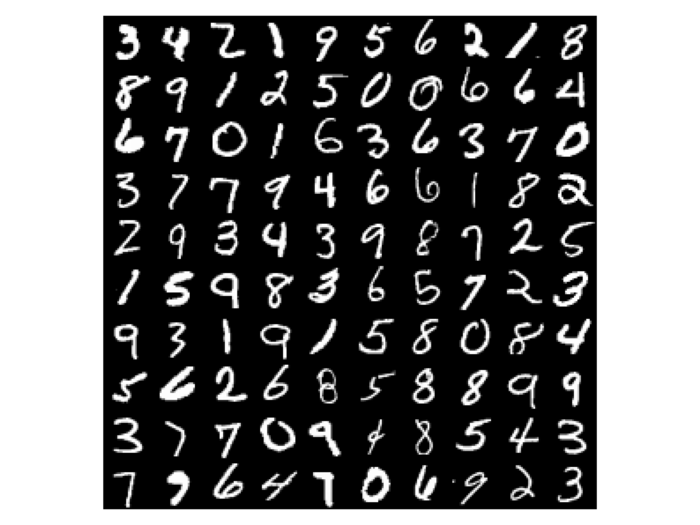
\includegraphics[width=0.7\textwidth]{imgs/mnist.png} 
    \caption{A figure.}
	\label{fig:test}
\end{figure}

\section{Experiments}

We orient our experiments primarily on the strip dataset, due to time and computational constrains.

After evaluating our models on the strip dataset, we look on the performance on other datasets for comparison and generalization.     

\subsection{Computational Constrains}

\subsection{Conversion comparison}

\subsection{Convolution vs no Convolution}

\subsection{Lateral connections}

\subsection{Hidden sparsity/ learning the data distribution}

\subsection{Same number of samples}

 